%% Author_tex.tex
%% V1.0
%% 2012/13/12
%% developed by Techset
%%
%% This file describes the coding for modeloLEA.cls

\documentclass[a4paper]{modeloLEA} %%%% where modeloLEA is the template name

\usepackage[portuguese]{babel}
\usepackage[T1]{fontenc}
\usepackage[utf8]{inputenc}
\usepackage{fancyhdr}
\usepackage{icomma}
\usepackage{booktabs}

\pagestyle{fancy}
\renewcommand{\headrulewidth}{0pt}
\fancyhead[L]{}
\fancyhead[C]{}
\fancyhead[R]{}

\usepackage{indentfirst}
\usepackage{booktabs}
\usepackage{graphicx}



%%%% *** Do not adjust lengths that control margins, column widths, etc. ***

%%%%%%%%%%% Defining Enunciations  %%%%%%%%%%%
\newtheorem{theorem}{\bf Teorema}[section]
\newtheorem{condition}{\bf Condição}[section]
\newtheorem{corollary}{\bf Corolário}[section]
%%%%%%%%%%%%%%%%%%%%%%%%%%%%%%%%%%%%%%%%%%%%%%%

\usepackage{titlesec}
\renewcommand{\thesection}{\arabic{section}}
\renewcommand{\thesubsection}{\thesection.\arabic{subsection}}
\renewcommand{\thesubsubsection}{\thesubsection.\arabic{subsubsection}}


\begin{document}

%%%% Article title to be placed here
\title{Análise descritiva dos casos de oncologia no SUS em Maringá-PR}

\author{
Makson Pedro Rodrigues$^{a,b}$,
Emanuel Carneiro F. da Silva$^{a,b}$,
Vanessa Midori Kurata$^{c,d}$,
Andressa Nunes Siroky$^{a,e}$}

\address{
  $^{a}$Departamento de Estatística - UFRN\\
  $^{b}$Consultor\\
  $^{c}$Prefeitura Municipal de Maringá\\
  $^{d}$Consulente\\
  $^{e}$Orientação}
%%%% Subject entries to be placed here %%%%
\subject{
Estatística Aplicada à Saúde}

%%%% Keyword entries to be placed here %%%%
\keywords{
Estatística descritiva,
Sistema único de Saúde (SUS),
Oncologia}

%%%% Insert corresponding author and its email address}
%\corres{
%  \\
%  e-mail: 
%}

%%%% Abstract text to be placed here %%%%%%%%%%%%
\begin{abstract}
Este relatório apresenta uma análise descritiva dos dados relacionados aos casos de oncologia nos serviços de saúde do Sistema Único de Saúde (SUS) em Maringá-PR e proximidades, com o objetivo de oferecer uma visão mais clara e panorâmica do sistema.
\end{abstract}
%%%%%%%%%%%%%%%%%%%%%%%%%%%

%% Some pieces required from the pandoc template
\providecommand{\tightlist}{%
  \setlength{\itemsep}{0pt}\setlength{\parskip}{0pt}}
\providecommand{\EndFirstPage}{%
}

\maketitle

\section{Objetivos}\label{objetivos}

No Brasil, o Sistema Único de Saúde (SUS) constitui a principal porta de acesso da população aos serviços de saúde, abrangendo desde ações preventivas até o tratamento de doenças complexas, como o câncer. A análise de dados desempenha papel fundamental na identificação de padrões em saúde pública, possibilitando a elaboração de estratégias mais eficientes para a gestão adequada dos recursos \cite{livroSUS}.

O presente relatório tem como objetivo realizar uma análise descritiva de informações relacionadas à oncologia no SUS, com foco na cidade de Maringá-PR e regiões vizinhas, durante o ano de \textbf{2024}. A partir de bases de dados públicos fornecidas pela consulente, foram exploradas variáveis como número de casos diagnosticados, início de tratamento, valores aprovados mensalmente, municípios com mais casos, tipos de câncer registrados, estágios da doença e distribuição por faixa etária e sexo. O intuito principal é oferecer uma visão clara e acessível sobre o cenário regional do atendimento oncológico no período avaliado, auxiliando na identificação de padrões relevantes.

\section{Metodologia}\label{metodologia}

O conjunto de dados fornecido pela consulente abrange 58 municípios, dos quais apenas Maringá possui hospitais habilitados para o tratamento oncológico, sendos eles Hospital do Câncer e Hospital de Santa Rita. As demais cidades, por serem de menor porte, encaminham seus pacientes para esses dois centros de referência. A distribuição geográfica dos municípios analisados pode ser visualizada na Figura \ref{fig:mapa}.

\begin{figure}[h]

{\centering 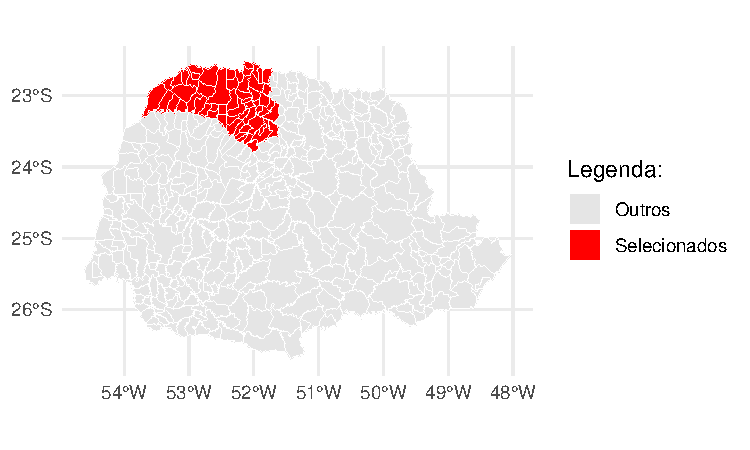
\includegraphics{relatorio_files/figure-latex/mapa-1} 

}

\caption{\label{fig:mapa}Mapa dos municípios do estado do Paraná.}\label{fig:mapa}
\end{figure}

Toda a análise foi conduzida com o uso da linguagem R \cite{R2017}, por possuir funções úteis para elaboração de gráficos, tabelas e estatísticas mais personalizadas, os dados analisados abrangem informações sobre faixa etária, sexo, número de estadiamentos, tipos de câncer e outras variáveis mensais, como número de diagnósticos, inícios de tratamento e valores aprovados pelo Estado. É importante destacar que todas essas variáveis estão segmentadas por município.

Um dos objetivos da consultoria era realizar uma análise envoltória \cite{livro}, uma metodologia que avalia a eficiência comparativa de unidades, baseando-se em múltiplos insumos e produtos. Todavia, essa análise não pôde ser realizada devido à limitação de dados disponíveis.

Também foram fornecidos dados detalhados sobre o Hospital do câncer e Hospital de Santa Rita, com o objetivo de realizar uma análise envoltória -- ou seja, avaliar a eficiência de cada unidade hospitalar considerando variáveis como salários médicos, número de leitos, equipe de enfermagem, casos mensais, tempo de espera, entre outros indicadores. No entanto, para que essa análise seja mais robusta e comparável, é necessário dispor de uma base de dados mais ampla, composta por diversos hospitais oncológicos a nível nacional.

\section{Resultados}\label{resultados}

Iniciando pela análise de variáveis mais identitárias, como sexo e idade (Figuras \ref{fig:sexo} e \ref{fig:idade}, respectivamente), observa-se nestes dados que há mais casos de câncer em mulheres. Apenas 13 municípios registraram um número maior de casos em homens. Além disso, como já era esperado, a maioria dos diagnósticos ocorreu entre pessoas mais velhas.

\begin{figure}[h]

{\centering 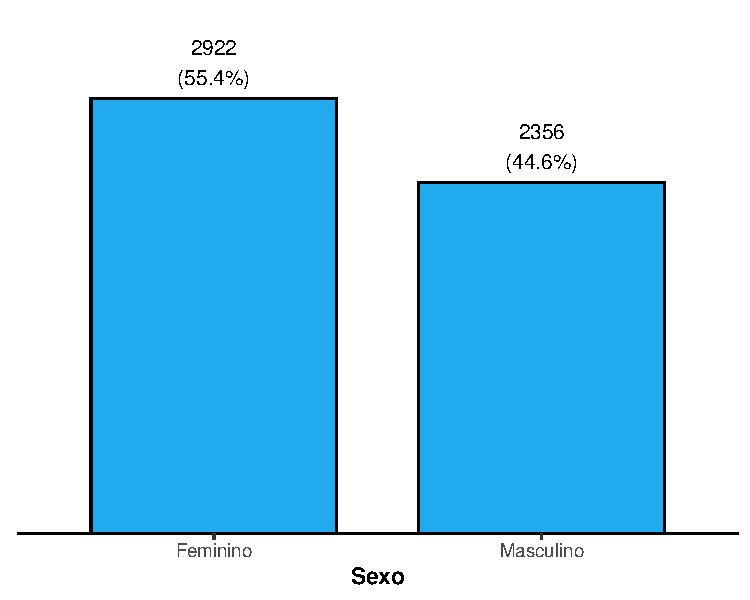
\includegraphics{relatorio_files/figure-latex/sexo-1} 

}

\caption{\label{fig:sexo}Número de casos totais de câncer por sexo.}\label{fig:sexo}
\end{figure}

\begin{figure}[h]

{\centering 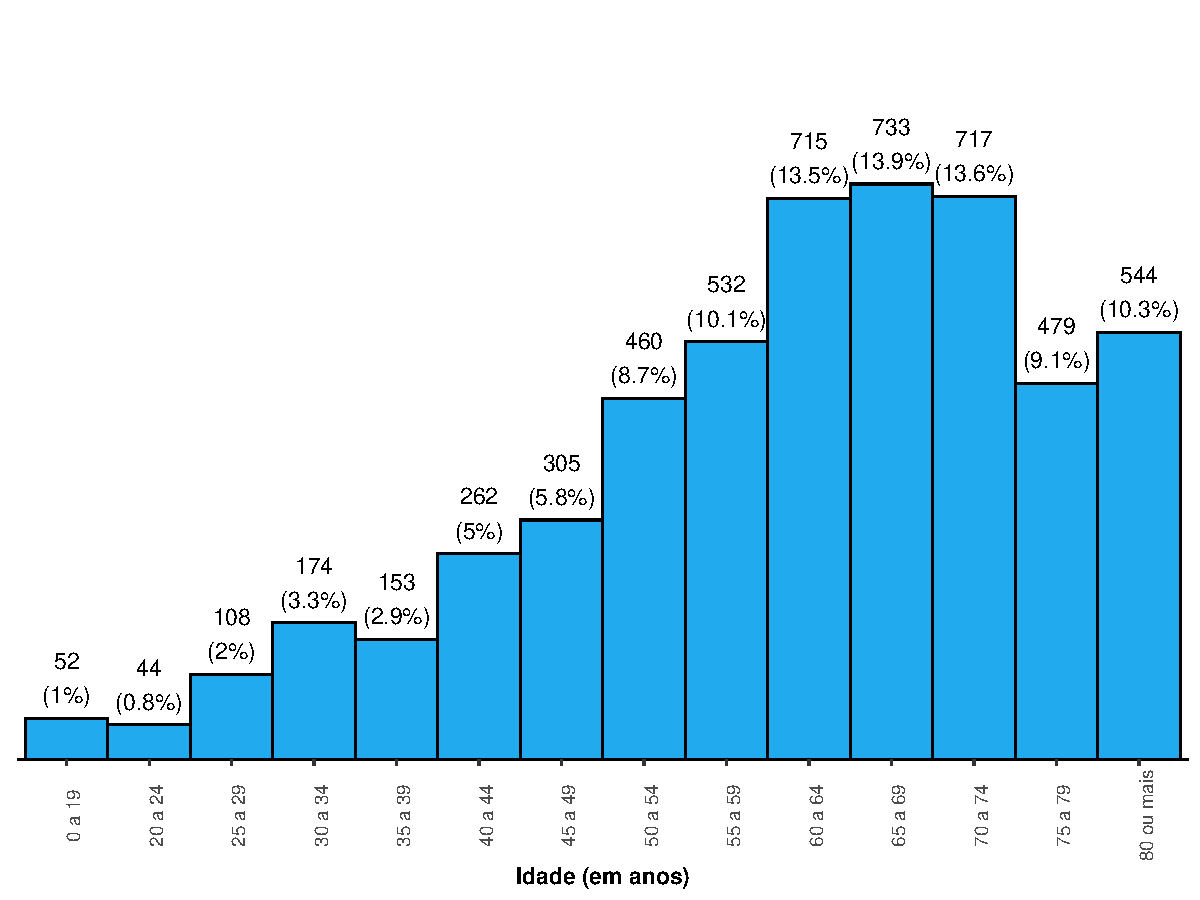
\includegraphics[width=0.8\linewidth]{relatorio_files/figure-latex/idade-1} 

}

\caption{\label{fig:idade}Número de casos totais de câncer por idade.}\label{fig:idade}
\end{figure}

\newpage

Agora, observa-se na tabela abaixo os municípios com maior concentração de casos oncológicos, bem como a porcentagem que cada um representa no total da região.

\begin{table}[!h]
\centering
\caption{\label{tab:municipios}Municípios com maior número de casos de câncer em 2024.}
\centering
\resizebox{\ifdim\width>\linewidth\linewidth\else\width\fi}{!}{
\fontsize{10}{12}\selectfont
\begin{tabular}[t]{lcc}
\toprule
Município & Porcentagem (\%) & Total de casos\\
\midrule
Maringá & 35,2\% & 1858\\
Paranavaí & 7,96\% & 420\\
Sarandi & 6,61\% & 349\\
Marialva & 3,90\% & 206\\
Paiçandu & 3,83\% & 202\\
\bottomrule
\end{tabular}}
\end{table}

A seguir, nas Tabelas 2 e 3, os dez tipos de câncer com mais casos diagnosticados em 2024 em toda região e também, exclusivamente, em Maringá.

\newpage

\begin{table}[!h]
\centering
\caption{\label{tab:tabela2}Dez tipos de câncer mais frequentes na região em 2024.}
\centering
\resizebox{\ifdim\width>\linewidth\linewidth\else\width\fi}{!}{
\fontsize{10}{12}\selectfont
\begin{tabular}[t]{lcc}
\toprule
Tipo de câncer & Total de casos & Porcentagem (\%)\\
\midrule
Incerto/desconhecido & 1301 & 36\%\\
Outras neoplasias da pele & 771 & 21.4\%\\
Mama & 436 & 12.1\%\\
Próstata & 242 & 6.7\%\\
Cólon & 191 & 5.3\%\\
\addlinespace
Sem localização específica & 186 & 5.2\%\\
In situ do colo do útero & 141 & 3.9\%\\
Colo do útero & 131 & 3.6\%\\
Reto & 105 & 2.9\%\\
Outras neoplasias de comportamento incerto & 105 & 2.9\%\\
\bottomrule
\end{tabular}}
\end{table}

\begin{table}[!h]
\centering
\caption{\label{tab:tabela3}Dez tipos de câncer mais frequentes em Maringá em 2024.}
\centering
\resizebox{\ifdim\width>\linewidth\linewidth\else\width\fi}{!}{
\fontsize{10}{12}\selectfont
\begin{tabular}[t]{lcc}
\toprule
Tipo de câncer & Total de casos & Porcentagem (\%)\\
\midrule
Incerto/desconhecido & 539 & 39.6\%\\
Outras neoplasias da pele & 271 & 19.9\%\\
Mama & 164 & 12\%\\
Próstata & 89 & 6.5\%\\
Cólon & 75 & 5.5\%\\
\addlinespace
In situ do colo do útero & 53 & 3.9\%\\
Sem localização específica & 52 & 3.8\%\\
Metástase em gânglios linfáticos & 47 & 3.5\%\\
Pulmões e brônquios & 38 & 2.8\%\\
Colo do útero & 34 & 2.5\%\\
\bottomrule
\end{tabular}}
\end{table}

\vspace{1cm}

A Tabela 4 mostra quais estágios do câncer foram os mais comuns. O estágio 0 representa o início da doença, enquanto o estágio 4 indica uma fase mais avançada e grave. Percebe-se que os estágios mais iniciais da doença não são muito identificados, se diagnostiscando apenas quando se agrava.

\begin{table}[!h]
\centering
\caption{\label{tab:estagios}Número de casos de câncer em 2024 por estágio (Total e Maringá).}
\centering
\resizebox{\ifdim\width>\linewidth\linewidth\else\width\fi}{!}{
\fontsize{10}{12}\selectfont
\begin{tabular}[t]{lccc}
\toprule
Município & Estágio do câncer & Número de casos & Porcentagem (\%)\\
\midrule
Total & Estágio 0 & 56 & 5.5\%\\
Total & Estágio 1 & 80 & 7.9\%\\
Total & Estágio 2 & 296 & 29.2\%\\
Total & Estágio 3 & 324 & 32.0\%\\
Total & Estágio 4 & 257 & 25.4\%\\
\addlinespace
Maringá & Estágio 0 & 13 & 3.5\%\\
Maringá & Estágio 1 & 32 & 8.7\%\\
Maringá & Estágio 2 & 114 & 31.1\%\\
Maringá & Estágio 3 & 121 & 33.0\%\\
Maringá & Estágio 4 & 87 & 23.7\%\\
\bottomrule
\end{tabular}}
\end{table}

\newpage

As Figuras \ref{fig:diagnostico1} e \ref{fig:diagmaringa} apresentam gráficos de linhas comparando o número de casos diagnosticados com o número de inícios de tratamento ao longo dos meses de 2024. Observa-se que, em grande parte do período, o número de diagnósticos é bem superior ao de tratamentos iniciados, indicando uma defasagem entre detecção e início do tratamento. No entanto, essa diferença reduz-se bastante nos últimos meses do ano, sugerindo uma melhora na agilidade do sistema de atendimento.

\begin{figure}[h]

{\centering 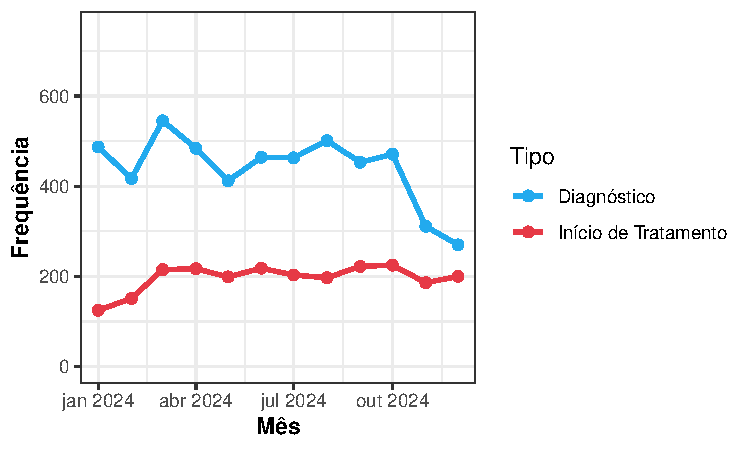
\includegraphics{relatorio_files/figure-latex/diagnostico1-1} 

}

\caption{\label{fig:diagnostico1}Número de diagnósticos e inícios de tratamento por mês.}\label{fig:diagnostico1}
\end{figure}

\begin{figure}[h]

{\centering 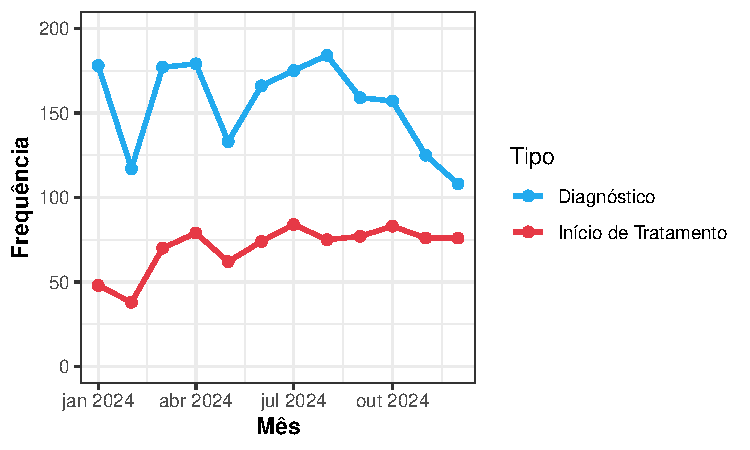
\includegraphics{relatorio_files/figure-latex/diagmaringa-1} 

}

\caption{\label{fig:diagmaringa}Número de diagnósticos e inícios de tratamento por mês (apenas Maringá).}\label{fig:diagmaringa}
\end{figure}

\newpage

Por fim, como mostram as Figuras \ref{fig:custo} e \ref{fig:custo2}, é nítido perceber uma queda no valor aprovado pelo Estado em abril de 2024. Isso aconteceu, em parte, por causa da redução em Maringá, que foi de pouco mais de R\$ 100 mil. No mês seguinte, no entanto, os valores já voltaram a subir. Nos meses seguintes, o custo total continuou aumentando, influenciado também pelo crescimento nos demais municípios. Na Figura \ref{fig:dispersao1}, percebe-se que a relação número de casos com valor aprovado é linear, com correlação consideravelmente próxima de 1 (aproximadamente 0,996), indicando uma distribuição de ementas proporcionalmente lineares.

\begin{figure}[h]

{\centering 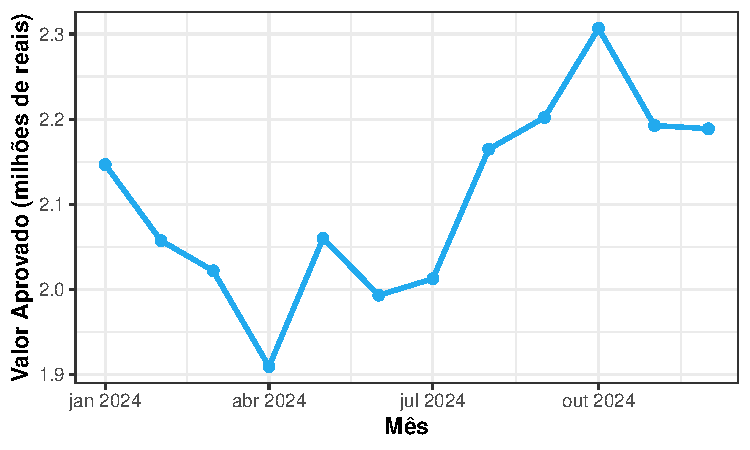
\includegraphics{relatorio_files/figure-latex/custo-1} 

}

\caption{\label{fig:custo}Valor total aprovado pelo governo para realização de consultas e tratamentos oncológicos.}\label{fig:custo}
\end{figure}

\begin{figure}[h]

{\centering 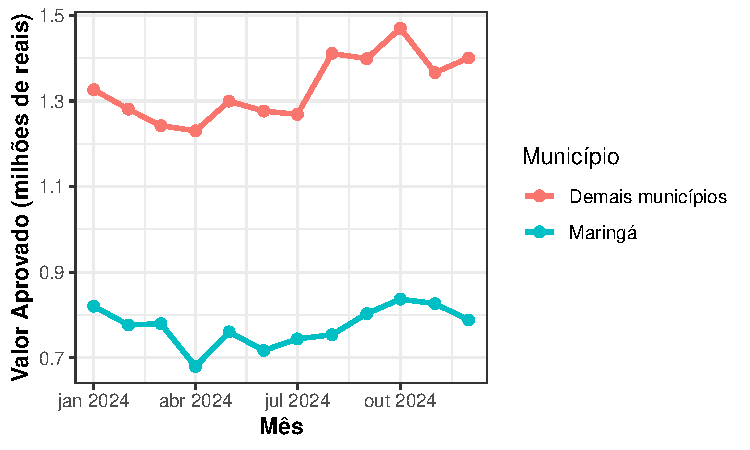
\includegraphics{relatorio_files/figure-latex/custo2-1} 

}

\caption{\label{fig:custo2}Valores aprovados pelo governo para realização de consultas e tratamentos oncológicos: Comparação entre Maringá e os demais municípios (excluindo Maringá).}\label{fig:custo2}
\end{figure}

\begin{figure}[h]

{\centering 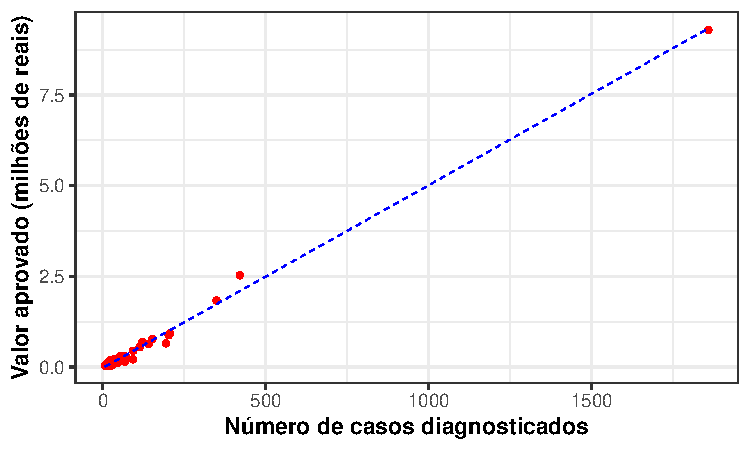
\includegraphics{relatorio_files/figure-latex/dispersao1-1} 

}

\caption{\label{fig:dispersao1}Número de casos diagnosticados vs Valor aprovado (por município em 2024).}\label{fig:dispersao1}
\end{figure}

\begin{table}[!h]
\centering
\caption{\label{tab:media}Média de valor aprovado por caso oncológico: maior, menor e geral da região.}
\centering
\resizebox{\ifdim\width>\linewidth\linewidth\else\width\fi}{!}{
\fontsize{10}{12}\selectfont
\begin{tabular}[t]{lccc}
\toprule
Município & Número de casos & Valor total aprovado & Média por caso\\
\midrule
Itaguaje & 22 & R\$ 180.106 & R\$ 8.187\\
Presidente Castelo Branco & 27 & R\$ 45.002 & R\$ 1.667\\
Geral (região) & 5278 & R\$ 25.257.642 & R\$ 4.785\\
\bottomrule
\end{tabular}}
\end{table}

O ponto em destaque na Figura (\ref{fig:dispersao1}) é Maringá, que se destaca pelo alto número de casos e, consequentemente, pelo alto valor. Mesmo assim, ele segue a tendência de correlação linear observada na dispersão dos dados. Na Tabela 5, mostra a média de gasto por caso, o valor chegou a R\$ 4.785,00 aprovados por caso oncológico. A cidade de Itaguajé detém a maior média dentre a região, sendo a única a alcançar R\$ 8.187,00, e a cidade com menor média foi Presidente Castelo Branco com média de R\$ 1.667,00.

\newpage

\textbf{Importante}: As escalas dos gráficos nas Figuras (\ref{fig:custo}) e (\ref{fig:custo2}) não iniciam no zero no eixo y, com o propósito de destacar melhor as diferenças de custo. Essa decisão se justifica pelo fato de que os custos analisados são todos superiores a um milhão de reais, enquanto as variações entre eles costumam ser pequenas. Iniciar o eixo em zero dificultaria a visualização dessas variações sutis, que são relevantes para a análise.

\section{Conclusões}\label{conclusuxf5es}

Com base nas tabelas e gráficos apresentados, é possível afirmar que uma análise mais aprofundada, como a aplicação de modelos de séries temporais para observar a variação no número de diagnósticos e tratamentos ao longo dos meses, exigiria um conjunto de dados mais completo. O ideal seria contar com informações de um período maior, além de dados de outras regiões do Paraná ou até mesmo de outros estados, permitindo comparações mais amplas e melhores. Essa mesma necessidade se aplica a uma análise envoltória de dados (DEA), que depende da diversidade e abrangência das informações dos hospitais para gerar resultados mais confiáveis.

No geral, como era de se esperar, Maringá se destaca com um valor aprovado pelo Estado bem mais alto do que os demais municípios da região, concentrando cerca de 35\% dos casos. Por isso, ele recebeu mais atenção nas análises. Outro ponto que vale destacar é que, nos últimos meses do ano, a diferença entre os diagnósticos de câncer e os inícios de tratamento foi consideravelmente menor.







\bibliographystyle{RS}
\bibliography{modeloLEA.bib}


\end{document}
